\chapter{Implementation}
\label{chap:implementation}

\section{Tools and Libraries}

\begin{enumerate}
    \setlength\itemsep{-1.05em}
    \item \textbf{Python 3.11.11}: The version of Python used for the development environment.
    \item \textbf{Jupyter Notebook}: A web-based interactive computing environment to write and execute code.
    \item \textbf{VS Code}: A source-code editor used for writing and editing the project code.
    \item \textbf{Kaggle for Fine-Tuning}: Platform used for training models on large datasets.
\end{enumerate}

\subsection*{Data Handling Libraries}
\begin{enumerate}
    \setlength\itemsep{-1.05em}
    \item \textbf{datasets}: A library for accessing and managing datasets, particularly those used for machine learning tasks.
    \item \textbf{pandas}: Data manipulation and analysis library, used for handling data in tabular form.
    \item \textbf{numpy}: Provides support for large multi-dimensional arrays and matrices, along with a collection of mathematical functions to operate on them.
    \item \textbf{faiss}: A library for efficient similarity search and clustering of dense vectors.
\end{enumerate}

\subsection*{Deep Learning Frameworks}
\begin{enumerate}
    \setlength\itemsep{-1.05em}
    \item \textbf{lightning}: A lightweight PyTorch wrapper for high-performance, multi-GPU, and distributed training.
    \item \textbf{torch}: PyTorch, an open-source deep learning framework for tensor computation and building neural networks.
    \item \textbf{torchvision}: A library containing datasets, model architectures, and image transformations for computer vision.
    \item \textbf{tensorflow}: An open-source machine learning framework used for training deep learning models (used alongside PyTorch in this case).
\end{enumerate}

\subsection*{Computer Vision Libraries}
\begin{enumerate}
    \setlength\itemsep{-1.05em}
    \item \textbf{opencv-python}: A Python wrapper for OpenCV, a library used for real-time computer vision and image processing tasks.
    \item \textbf{opencv-python-headless}: A version of OpenCV without GUI functionality, used in headless environments.
\end{enumerate}

\subsection*{Miscellaneous Libraries}
\begin{enumerate}
    \setlength\itemsep{-1.05em}
    \item \textbf{albumentations}: A library for fast and flexible image augmentations.
    \item \textbf{PIL (Pillow)}: A library used for opening, manipulating, and saving many different image file formats.
    \item \textbf{fashion-clip}: A specialized library used for fashion-related image and text embeddings.
    \item \textbf{streamlit}: A tool to quickly build web apps for machine learning and data science projects.
    \item \textbf{sqlalchemy}: A database toolkit for Python that provides an ORM (Object-Relational Mapping) system.
    \item \textbf{psycopg2-binary}: PostgreSQL adapter for Python.
    \item \textbf{alembic}: A database migration tool for SQLAlchemy.
    \item \textbf{pydantic}: Data validation and settings management library.
    \item \textbf{python-dotenv}: A library to load environment variables from `.env` files.
    \item \textbf{google-generativeai}: A library for integrating with Google's generative AI models.
\end{enumerate}

\subsection*{Development and Testing Libraries}
\begin{enumerate}
    \setlength\itemsep{-1.05em}
    \item \textbf{ipykernel}: The Python kernel for Jupyter.
    \item \textbf{scikit-learn}: A machine learning library for Python that provides simple and efficient tools for data mining and data analysis.
    \item \textbf{tqdm}: A library for showing progress bars in Python loops.
    \item \textbf{requests}: A simple HTTP library for making requests in Python.
\end{enumerate}

\section{Fine-Tuning Process}

\subsection*{Collator Function}
In the fine-tuning process, we use a collator function that takes a batch of input dictionaries and transforms them into a dictionary where each key's value is a vector, facilitating the training of the model with batches.

\vspace{-1.25em}
The \texttt{collate\_fn} function pads the input images to a fixed size and processes the labels, including boxes, areas, and class labels, before returning them in a structured format suitable for feeding into the model.

\vspace{-1.25em}
\subsection*{DataLoader}
A DataLoader is used to load batches of the prepared dataset. It feeds the dataset into the model during training and validation. The \texttt{train\_dataloader} and \texttt{val\_dataloader} are set up with the batch size, and the collator function to ensure that data is correctly formatted.

\vspace{-1.25em}
\subsection*{Model Definition}
PyTorch Lightning is used for defining and training the model. In the model class, we define the architecture, including the pre-trained YOLOS model for object detection. The \texttt{Detr} class contains methods for forward propagation, common steps during training and validation, and the configuration of optimizers.

\vspace{-1.25em}
The model is designed to output both the predicted boxes and the loss values, which are then logged for monitoring the training progress.

\vspace{-1.25em}
\subsection*{Model Training}
The training process is initiated using PyTorch Lightning’s \texttt{Trainer} class. The \texttt{trainer.fit(model)} command starts the training process, specifying the number of epochs, accelerator, and device used.

\vspace{-1.25em}
\section*{Streamlit Implementation}

In the Streamlit implementation, we use a unified chat system where users can search for products using natural language queries or by uploading images. This system allows users to either perform a text-based or image-based search.

\vspace{-1.25em}
We use the \texttt{gemini} model for natural language processing to determine the type of search (text or image) and extract relevant information such as search terms or image links. The \texttt{infer\_query} function handles this by interpreting user input and returning a structured JSON response that includes the query type, number of results, search terms, and image URL if applicable.

\vspace{-1.25em}
\texttt{gemini} analyzes the user's query to determine whether they are asking for a text-based or image-based search, and then identifies the specific search term or image link. If no image link is provided, the function returns \texttt{None} for the image URL key.

\vspace{-1.25em}
The streamlit implementation can be summerized by the following diagram:
\begin{figure}[H]
    \centering
    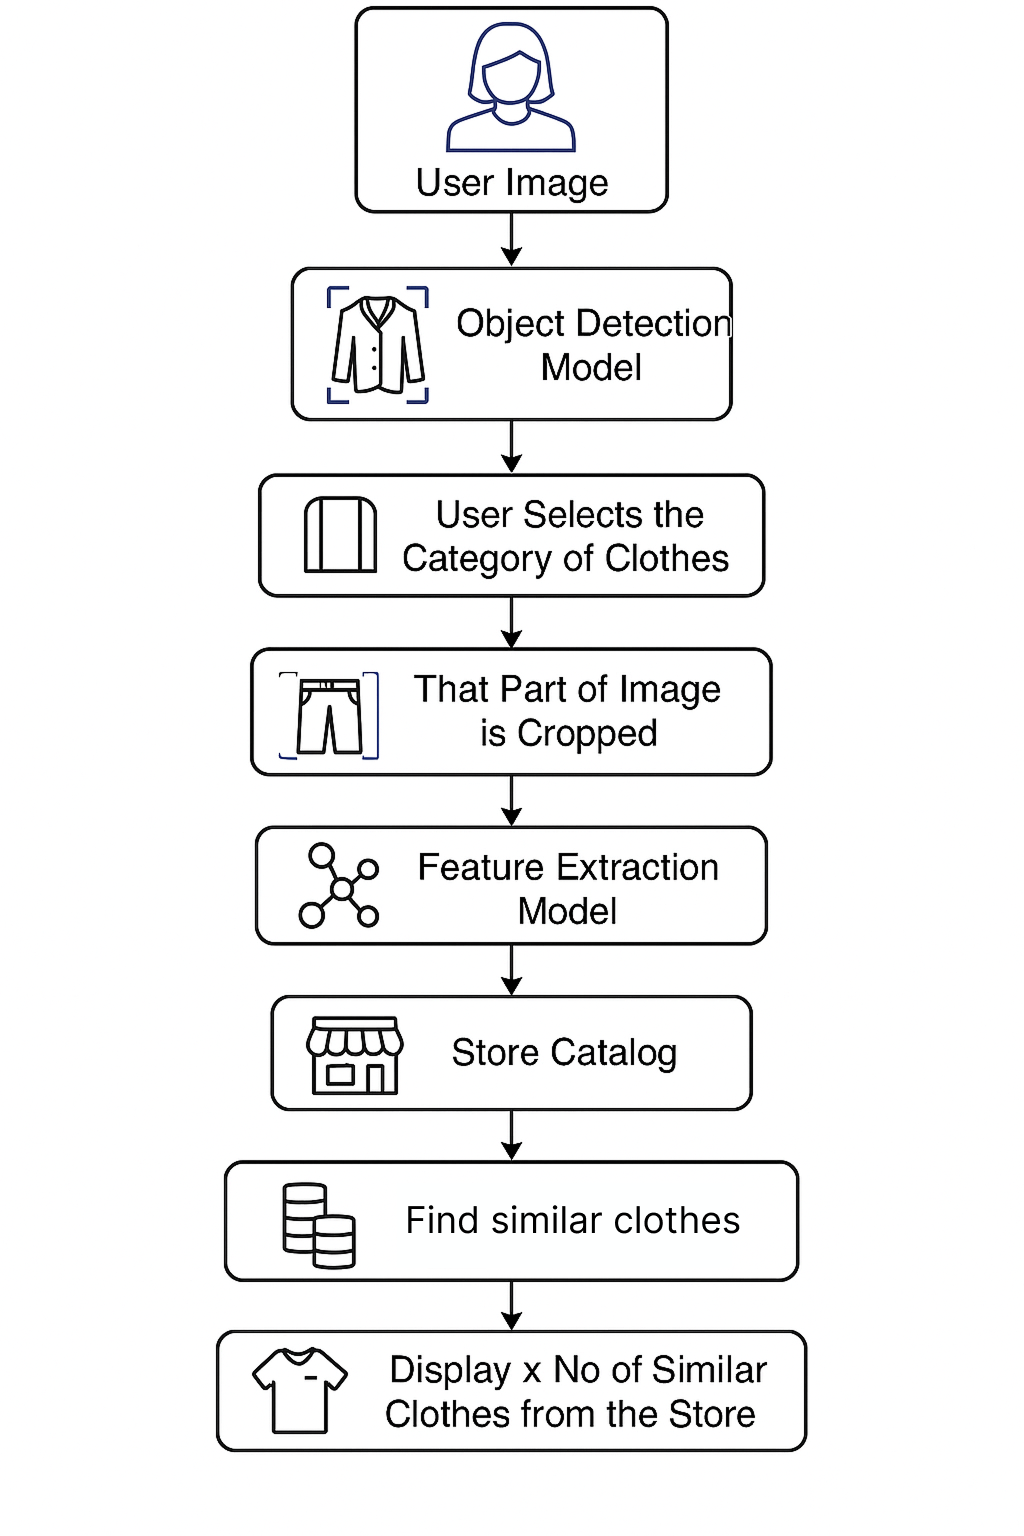
\includegraphics[width=0.4\textwidth]{images/workflow.png}
\end{figure}